%chapter 3
\chapter{Transportation Economics}
%
\section{Introduction}
All decisions related to planning, design, and improvement of transportation infrastructure have economic implications. Transport economics includes the issues such as transport location, movement of people and freight/goods, transport demand, transport planning and forecasting, direct and indirect cost of transport, pricing of transport services, investments in transport infrastructure and services, transport and social-economic development, and transport regulation. In this chapter the transport economics is considered from the micro economic perspective. We consider various aspects of the direct costs and pricing of transport infrastructure and services of different transportation modes.\\
\par
Considered from this microeconomic perspective, it can be said that the transport sector consists of the demand and supply component. The transport demand is derived demand due to needs of people and freight/goods shipments to change the physical place. For example, many people live at one place but work and/or have a leisure on the others, which requires them to travel forward and backward. The location of companies providing raw materials is different than those of the users of these materials—manufacturers of the semifinal and final products, which requires transportation of these raw materials from the former to the latter. In addition, the manufacturers of the final products are often located far away from the retailers of these products, which again require transportation, this time of the final products. Thus, it can be said that the transport demand is derived demand. In many cases transportation demand is proportional to the volumes of peoples’ activities and the quantities of final products they consume during a given period of time.\\
\par
The transport demand is handled by the transport supply/capacity provided by transport companies.
The transport companies generally provide transport infrastructure with the supportive facilities and equipment, and rolling stock/vehicles carrying out transport services. In order to make them operational, the corresponding material, labor, ie, employed staff/personnel, and energy/fuel, are consumed. In terms of time, the transport infrastructure has particularly the long life-cycle, which is, for example, about 20, 30, 40, or even 60 years. That of rolling stock/vehicles is shorter (20–25 years) mainly due to its/their physical and also technological obsolescence, after they need to be replaced. In this context, two categories of transport companies can be distinguished: that providing transport infrastructure called “the infrastructure providers,” and that providing transport services called “transport operators.” They both constitute the transport systems within particular transport modes.\\
\par
According to the economic jargon, the above-mentioned components of transport supply/capacity represent the main inputs to transport processes. The outputs of the transport process are the transport services produced in the given quantities and at the specified quality. They are consumed by users— passengers and/or freight shippers/receivers at the same time as they are produced. This implies that they are the short-lived similarly as transport demand without possibility to be stored/warehoused and left to be consumed sometimes latter on.\\
\par
The most important economic categories of a given transport system are its costs, revenues, and their relationship.\\
\par
The costs are expenses for maintaining the transport infrastructure and carrying out transport
services. These costs are passed to users of these services (passengers and freight/goods shippers and receivers) in the form of prices/charges. These charges bring revenues to transport companies. In general, these prices/charges, ie, revenues, are set up to cover the company’s costs and provide some profits. Nevertheless, the difference between revenues and costs can generally be positive or negative, thus representing the profits or losses. Profits or losses are calculated for the given period of time (usually for a quarter of year, year, or few years).\\
\par
The prices charged to users of transport services represent for them direct costs. In addition, users are imposed the indirect costs, which are usually considered to be the cost of time during trip/travel/ transportation. In such case, the sum of direct and indirect costs is called the users’ generalized trip/ travel/transportation costs for users.\\
\par
We describe in this chapter the main elements of economics of transportation systems considered
from the engineering perspective. The chapter analyzes direct costs and revenues of the providers of transport infrastructure and transport operators. Costs and revenues could be analyzed at the level of the individual component (infrastructure, rolling stock) and/or of the entire company.
%
\section{Scope of Transportation Economics}
The study of economics is divided into macro-economics and micro-economics. Macro-economics is associated with the wealth of society on a regional scale, and deals with the behavior of aggregate concepts. On the other hand, micro-economics involves the behavior of relatively smaller entities such as firms and individuals. Transportation economics, while considered a branch of applied micro-economics, is associated with certain unique issues such as:
\begin{enumerate}
	\item the demand for transportation is not direct, but is derived
	\item the consumption of each transportation facility (i.e., each trip) is unique in time and space
	\item technological differences among different modes and economies of scale
	\item governmental interventionist policies and regulations in transportation
\end{enumerate}
Transportation economics specifically addresses demand of transportation services, supply of transportation facilities, elasticity of demand and supply, price mechanisms, and transportation cost analysis
%
\section{Transportation Demand}
Like all other goods and services, the demand for any specific transportation facility demands on factors pertaining to the consumer such as income, and characteristics of the facility such as the cost associated with its use (in terms of time and price) relative to rival facilities. A typical example of such demand is that for auto travel: lower incomes of consumers, coupled with lower costs and travel times associated with transit are expected to lead to reduced demand for auto travel. Transportation demand analysis involves demand functions (which represents the willingness of consumers to purchase the transportation “product” at various alternative prices, i.e., the demand-price curve, and demand models (which estimate the probability that an individual (or fraction of a set of individuals) will choose a particular product over the other.
\paragraph{}
\begin{center}
	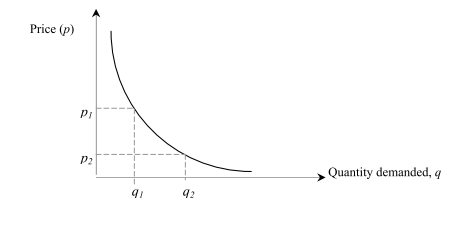
\includegraphics{gfx/fig38.png}
\end{center}
A hypothetical example of an aggregate transportation demand function is provided as shown in the above figure. This represents the amount of travel people are willing to make by transit at various transit fare (price) levels. Transportation demand functions, either in the form of a graph or an equation, are useful in transportation planning because they enable the determination of expected demand at any price. A specific demand curve represents the demand-price relationship given a set of conditions specific to the transportation product in question (referred to as alternative-specific attributes, such as travel time, comfort, convenience), and also specific to the users (income levels and other socioeconomic characteristics). Changes in such conditions often result in changes in the levels of transportation demand, even at fixed price of that product. For example, increased unemployment would likely lead to reduced demand for travel. Also, an increase in costs associated with auto use is likely to result in increased transit demand, even if transit fares remain the same. When such changes in conditions (other than price) occur, they are represented as a shift in the demand curve shown in the figure below (upward shift for increased demand, $ D_1 $ → $ D_2 $; and downward shift for decreased demand, $ D_1 $ → $ D_3 $).
\begin{center}
	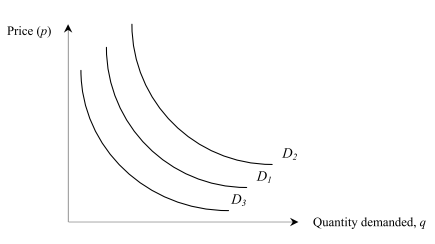
\includegraphics[scale=0.7]{gfx/fig39.png}
\end{center}
%
\subsection{Causes of Shift in Transportation Demand Curve}
There is a possibility of a change in demand of a transportation facility even when its price remains same, and this is reflected as a shift in the demand curve for that transportation facility. Factors that influence such demand shifts are discussed below:
\begin{itemize}
	\item \textit{\textbf{Sudden change in customer preference}}: (Season, life, style, e.t.c) For example, more people seem to ride transit in the winter season.
	\item \textit{\textbf{Change in the level of attribute of interest (e.g., increase in price) of related goods}}: For complementary products, a decrease in price of product increases the demand for other product, shifting the latter's demand curve to the right (e.g., parking spaces, automobile use). For rival products, an increase in price of a product increases the demand for its rival product, shifting the latter's demand curve to the right (e.g., transit, auto).
	\item \textit{\textbf{Change in regional income}}: An increase in income shifts the demand curve to the right. A normal good is one whose demand increases as a person's income increases.
	\item \textit{\textbf{Change in number of potential customers}}: An increase in market size shifts the demand curve towards right.
	\item \textit{\textbf{Expectation of impending change in the level of the attribute of interest}}: e.g., A news report predicting higher prices in the future can cause a shift in the demand curve at the current price as customers purchase increases in the anticipation of the price change.
\end{itemize}
%
\subsection{Transportation Demand Functions}
Transportation demand models are used to determine the volume of travel demanded, at various levels of service and have been described as “a representation of human behavior which can be used to predict how individuals or firms will change transportation choices in response to changes in future conditions”. Within the context of transportation economics, a trip maker is defined as a consumer, in the economics meaning of the word, as the trip maker, by planning a trip, seeks to consume the service offered by transportation facilities. There are two types of demand functions:
\begin{enumerate}
	\item \textit{Disaggregate demand functions}: These predict the behavior of a single consumer in response to changes in future conditions.
	\item \textit{Aggregate demand functions}: These predict the behavior of a group of consumers such s a household, in response to changes in future conditions.
\end{enumerate}
\subsubsection{Linear Demand Function}
\begin{center}
	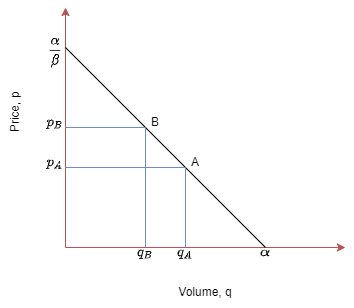
\includegraphics[scale=0.6]{gfx/fig40.png}
\end{center}
A linear demand function for travel as shown in the above figure for a given pair of origin and destination points, at a specific time of day and for a particular purpose. Such a demand function is useful for predicting travel over a wide range of conditions. This demand function is useful for predicting travel over a wide range of conditions. This demand function assumes a particular level and distribution of income, population, and socioeconomic characteristics. Note that it is an aggregate demand curve, representing the volume of trips demanded at different prices by a group of travelers. Functionally,
\begin{equation}
	q = \alpha - \beta p
	\label{linearDemandFunction}
\end{equation}
Where, q is the quantity of trips demanded, p is the price, and $\alpha$ and $\beta$ are constant demand parameters.The demand function is drawn with a negative slope expressing a similar situation where a decrease in perceived price usually results in an increase in travel, although it is not always true.
\begin{center}
	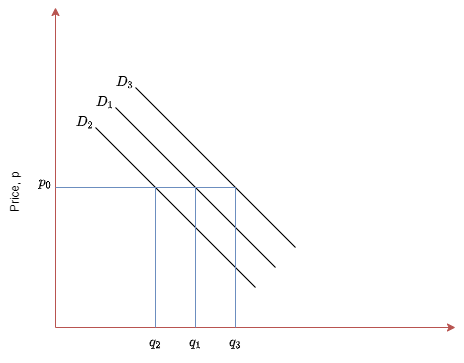
\includegraphics[scale=0.5]{gfx/fig41.png}
\end{center}
The above figure shows a series of shifted demand curves, representing changes in the quantity of travel due to variables other than the perceived price. Naturally, at a price $p_0$, one could expect different quantities $q_1$, $q_2$, and $q_3$ as the demand curve changes from $D_1$, $D_2$, and $D_3$. If the curve moves upward(from $D_1$ to $D_3$), it indicates an increase in trips.
\paragraph{}
It is important to distinguish short-run changes in the quantity of travel due to price changes represented by movement along a demand curve from long-run changes due to activity or behavioral variables, represented by shifts in demand functions.
%
\section{Transportation Supply}
\begin{center}
	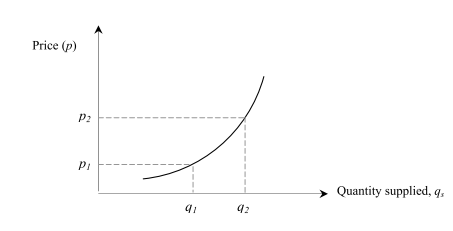
\includegraphics{gfx/fig42.png}
\end{center}
The supply of a transportation product represents the quantity of that product a producer is willing to offer at a given price. However, transportation supply may also be associated with the quality of the product. At a given time, transportation facility supply depends on price: higher prices are an incentive for producers to make more profits who therefore increase supply levels. A hypothetical example of a transportation supply function is provided as shown in the figure above. This represents the amount of transportation products that suppliers are willing to make available at various prices. Transportation supply functions are useful in transportation planning because they enable the determination of expected supply at any future price. A specific supply curve represents the supply-price relationship given a set of conditions specific to the transportation product in question (referred to as alternative-specific attributes, such as travel time, comfort, convenience), and also specific to the producers (such as technology, policy and governmental intervention through policies and regulation. Changes in such conditions often result in changes in the levels of transportation supply, even at fixed price of that product. For example, improved increased unemployment would likely lead to reduced demand for travel. Also, an increase in costs associated with auto use is likely to result in increased transit demand, even if transit fares remain the same. When such changes in conditions (other than price) occur, they are represented as a shift in the supply curve shown in the figure below (upward shift for increased demand, $ S_1 $ → $ S_2 $; and downward shift for decreased demand, $ S_1 $ → $ S_3 $).
\begin{center}
	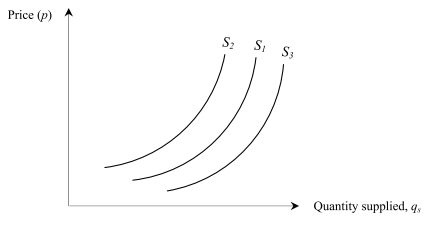
\includegraphics{gfx/fig43.png}
\end{center}
Increases in transportation supply may be traditionally thought of in terms of increasing the fleet size of a transit company or building new roads or increasing the number of lanes for existing roads. However, it is possible to increase supply without such physical capital-intensive investments. For instance, the use of intelligent transportation systems could lead to increased supply without any physical enlargements of the road network.
\subsection{Causes of Shift in Transportation Supply Curve}
The supply of transportation service may change even if the price remains constant, for reasons such as:
\begin{itemize}
	\item \textit{\textbf{Price of rival transportation services}}: The supply of a service may decrease if there is a decrease in the price of competing transportation service. This may apply to toll roads, where profit is the primary intent, and to a lesser extent, non-toll roads.
	\item \textit{\textbf{Number of transportation modes}}: An increased number of modes, such as construction of a subway in a city that already has buses and light rail transit and facilities for autos, indicates an increase in supply, shifting the supply curve towards right.
	\item \textit{\textbf{Price of relevant input}}: If the cost of resources used to produce a transportation service increases, the transportation agency would be less capable of supplying the same quantity at a given price, and the supply curve will shift towards left.
	\item \textit{\textbf{Technology}}: Technological advances that increase facility capacity or efficiency causes the supply curve to shift towards right.
\end{itemize}
%
\section{Equilibrium of Transportation Demand and Supply}
\begin{center}
	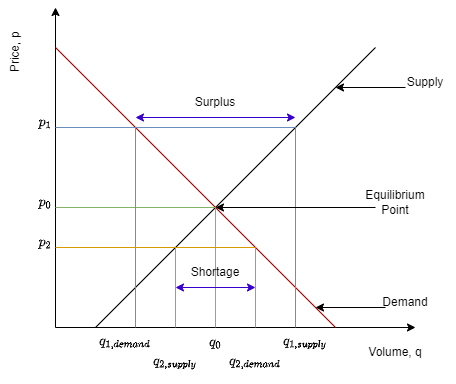
\includegraphics[scale=0.5]{gfx/fig44.png}
\end{center}
We have seen that the demand function is a relation between quantity demanded of a good and its price. Similarly, the supply function(Service function) represents the quantity of goods a producer is willing to offer at a given price. If the demand and supply function for a transportation facility are known, then it is possible to deal with the concept of equilibrium. Equilibrium is said to be attained when factors that affect the quantity demanded and those that determine the quantity supplied result in being statically equal (or converging toward equilibrium).\\\\
\textit{Numerical example:}\\
The travel time on a stretch of highway lane connecting two activity centers has been observed to follow the equation representing the service function:
$$ t = 15 + 0.02 v $$
Where t and v are measured in minutes and vehicles per hour respectively. The demand function for travel connecting the two activity centers is $ v = 4000 - 120t $.
\begin{itemize}
	\item Sketch these two equations and determine the equilibrium time and speed of travel.
	\item If the length of the highway lane is 20 miles, what is the average speed of vehicles traversing this length?
\end{itemize}
\textit{Solution:}\\\\
Demand function: $v = 4000 - 120t$\\
Supply function: v = 4000 - 120t\\
Solving these two equations simultaneously yields:\\\\
$v$ = 647 vehicles/hour\\
$t$ = 27.94 minutes\\\\
$ \therefore speed = \frac{20 \times 60}{27.94} = 42.95 mph$
\begin{center}
	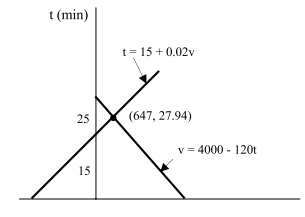
\includegraphics{gfx/fig45.png}
\end{center}
%
\section{Sensitivity of Travel Demand}
In the planning and evaluation of transportation systems and associated investments, it is often useful to have knowledge of the changes in transportation demand caused by changes in attributes of the transportation system or its environment. A particular instance is the change in demand for a given mode in response to changes in price of that mode. Given the functional form of the travel demand function, it is possible to derive a marginal effects model that estimates any one of the following:
\begin{itemize}
	\item Change in demand in response to unit change in attribute
	\item Change in demand in response to unit percent change in attribute
	\item Percent change in demand in response to unit percent change in attribute
\end{itemize}
The law of demand states that a fall in the price of a good raises the quantity demanded. The price elasticity of demand measures how much the quantity demanded responds to a change in price. Demand for a good is said to be elastic if the quantity demanded responds substantially to changes in the price. Demand is said to be inelastic if the quantity demanded responds only slightly to changes in the price.
\paragraph{}
Transportation demand elasticity may be defined as the degree of responsiveness of transportation demand in response to a unit change in demand-related or attributes such as price or income. This is typically expressed as follows:\\\\
$$ e_p =  \frac{percentage\; change\; in\; quantity\; demanded}{percentage\; change\; in\; price}$$
\begin{equation}
	e_p = \frac{\frac{\partial q}{q}}{\frac{\partial p}{p}} = \frac{\partial q}{\partial p} \times \frac{p}{q}
	\label{elasticity}
\end{equation}
Arc elasticity can be calculated as:
\begin{equation}
	Arc\; elasticity = \frac{\frac{\partial q}{q}}{\frac{\partial p}{p}} = \frac{\partial q}{\partial p} \times \frac{p}{q} = \frac{\frac{Q_1 - Q_0}{\frac{Q_1 + Q_0}{2}}}{\frac{P_1 - P_0}{\frac{P_1 + P_0}{2}}} = \frac{Q_1 - Q_0 \times (P_1 + P_0)/2}{P_1 - P_0 \times (Q_1 + Q_0)/2}
\end{equation}
Where, $Q_0$ and $Q_1$ represent quantity of travel demanded corresponding to prices $P_0$ and $P_1$ respectively.
\subsection{Elasticity and Revenue Along a Linear Demand Curve}
For a linear demand function, we can determine the elasticity of demand by taking derivative of equation \ref{linearDemandFunction}:
$$ \frac{dq}{dp} = - \beta$$
Also from equation \ref{linearDemandFunction},
$$ p =  \frac{\alpha - q}{\beta} $$
We have,
$$ e_p = \frac{\partial q}{\partial p} \times \frac{p}{q} $$
Substituting the values of $\frac{dq}{dp}$ and $p$ we get,
\begin{equation}
	\therefore \:e_p = -\beta \times \frac{\alpha - q}{\beta \: q} = 1 - \frac{\alpha}{q}
\end{equation}
When the elasticity is less than –1 (i.e., more negative than –1), the demand is described as being elastic, meaning that the resulting percentage change in quantity will be larger than the percentage change in price. In this case, demand is relatively sensitive to price change. However, when elasticity is between 0 and –1, the demand is described as being inelastic or relatively insensitive. These ranges are shown in the figure below:
\begin{center}
	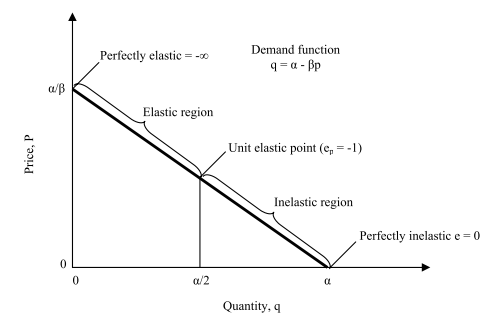
\includegraphics[scale=0.8]{gfx/fig46.png}
\end{center}
A linear demand curve has several interesting properties. Notice, as one moves down the the demand curve, the price elasticity of demand becomes smaller (i.e., more inelastic). In fact, the elasticity at a given point equals the length of the demand line segment below the point divided by the length of the line segment above it. Another point to is that the slope of the line is constant, but the elasticity changes from $\infty$ at the top, where the demand line intersects the vertical axis, ti $0$, where the demand line intersects the horizontal axis. Because elasticity changes along the demand curve, it is essential to specify what range of prices or quantity the elasticity was measured.\\\\
\begin{tabular}{|p{0.1\linewidth} | p{0.25\linewidth} | p{0.25\linewidth} | p{0.25\linewidth}|}
	\hline
	\textit{value} & \textit{Nature of Demand} & \textit{Relation between Price and Revenue} & Impact of increase in price\\
	\hline
	$ e > 1 $ & elastic & negatively related & reduces revenue\\
	$ e < 1 $ & inelastic & positively related & increases revenue\\
	$ e = 1 $ & unit elasticity & none & remains the same\\
	\hline
\end{tabular}
%
\section{Kraft Demand Function}
We occasionally come across a demand function where the elasticity of demand for travel with respect to its price is essentially constant. The demand function for such a situation corresponds to the equation.
\begin{equation}
	Q = \alpha (p)^\beta
	\label{kraftModel}
\end{equation}
Where $\alpha$ and $\beta$ are constant parameters of the demand function. To prove that this function is has a constant elasticity, we differentiate this function with respect to price, we get:
$$ \frac{dQ}{dp} = \alpha \: \beta \: p^{\beta - 1}$$
Now substituting this value in standard elasticity equation \ref{elasticity},
$$ e_p = \frac{dQ}{dp} \times \frac{p}{Q}$$
$$= \alpha \: \beta \: p^{\beta - 1} \times \frac{p}{Q}$$
$$= \alpha \: \beta \: p^{\beta - 1} \times \frac{p}{\alpha (p)^\beta} \: \: [from \: equation \: \ref{kraftModel}]$$
\begin{equation}
	\therefore e_p = \beta
\end{equation}
Thus, $\beta$, the exponent of price (a constant parameter), is the price elasticity.\\\\
\textit{Numerical Example:}\\
The elasticity of transit demand with respect to price has been found to be equal to -2.75, which means that a 1\% increase in transit fare will result in 2.75 decrease in the number of passengers using the system. A transit line on this system carries 12,500 passengers per day, charging 50 cents per ride. The management wants to raise the fare to 70 cents per ride. What advice would you offer to the management?\\
\textit{Solution}:\\
Since the elasticity of the demand is a constant, the demand function is a Kraft Demand Model,\\\\
$Q_1$ = 12500\\
$p_1$ = 50\\
$p_2$ = 70\\
$\beta$ = -2.75\\\\
We have,\\
$ Q_1 = \alpha (p_1)^\beta$\\
$ 12500 = \alpha \times 50^{-2.75}$\\
$\therefore \alpha = 5.876 \times 10^{8}$\\\\
An increase in fare from 50 to 70 cents will attract a demand of,\\\\
$ Q_2 = \alpha (p_2)^\beta$\\
$ \therefore Q_2 = 5.876 \times 10^{8} \times 70^{-2.75} \: = 4955 \: passengers$\\\\
Therefore, the increase in fare from 50 to 70 cents (40\% increase) is likely to reduce the patronage on this line from 12500 passengers per day to 4955 (60 \% decrease). In terms of revenue, the results are as follows:\\\\
Revenue before increase in fare ($R_1$) = 50 $\times$ 12500 = \$6250\\
Revenue after increase in fare ($R_2$) = 70 $\times$ 4955 = \$3468.50\\
$\therefore$ Loss in revenue = $ R_1 - R_2$ = \$6250 - \$3468.50 = \$3406\\\\
Hence, the management is not advised to increase the fare.
%
\section{Transportation Projects Evaluation}
Construction of highways along with the other associated infrastructures, construction of a new freight center, acquisition of new vehicles for the transit e.t.c. represent transportation projects faced by transportation experts. In the initial stage of these projects, it is necessary to perform their evaluation, that is, as precise as possible, analyze and review economic, environmental, equity, as well as other project impacts. The planners and engineers must properly answer the following questions: (a) Are the transportation project’s benefits greater than the projects’ costs?; (b) What is the best project’s alternative in the case when project has few mutually exclusive alternatives?; (c) How to allocate available funds among competitive transportation projects?; (d) When to start the considered project?\\
\par
Frequently, financial resources are scarce, and appropriate engineering economic analysis can significantly help planners and decision-makers to allocate available resources properly. In the first step ofany project evaluation, it is necessary to analyze the project’s socio-economic context, and to clearly define the project’s objectives. In the next steps, the analysts should clearly recognize the type of costs and benefits, compare them and make recommendations to the decision makers.\\
\par
Transportation projects usually extend over many years. On the other hand, the purchasing power of money decreases over time. The main cause of this phenomenon is the inflation that exists in every society. A discount rate regulates the value ofmoney for time. This rate is used to represent future monetary quantities in terms oftheir today’s value. Compounding and discounting are techniques that enable us to compare money values at different points in time. Let us briefly explain compounding technique.\\
\par
Let us assume that we want to invest \$100 these days, at an annual interest rate (r) of 5\%. It will be \$100 + \$5 = \$105 in 1 year. After two years it will be 105\$ + \$0.05 * 105 = \$110.25. After 3 years we will have \$110.25 + \$0.05 * \$110.25 = \$115.7625. Discounting represent reverse operation of compounding. The compounding technique helps us to find the answer to the following question: what is the present value $(PV)$ of a known future amount of money?\\
\par
In our example, the $PV$ of \$105 next year, when $r$ = 5\%, is \$100. The $PV$ equals
\begin{equation}
	PV = V_t/(1 + r)^t \; \; t = 0, 1, 2,......,n
\end{equation}
Where $n$ is the project duration (in years), $r$ is the rate of discount, and $V_t$ is the value in year $t$.\\
\par
There are two interest rates that are used in transportation projects evaluation. The first one is the real interest rate that is exclusive of inflation, while the second one is the nominal interest rate that is inclusive of inflation. Project value is usually expressed as a NPV. This value represents a project’s value or cost for its whole life cycle in today’s dollars.\\
\par
When evaluating transportation projects many governments and funding agencies in the world (OECD, World Bank, etc.) require a cost-benefit analysis (CBA) to be performed. In this way, the CBA represents common evaluation language between the governments, funding agencies and the transportation project supporters.\\
\section{Cost-Benefit Analysis}
The CBA is a method that calculate and compare project’s costs and benefits to society over period of time. The CBA monetizes all project’s inputs and outputs. In other words, the CBA converts the inputs and the outputs into a monetary values. The CBA helps decision-makers to rank and prioritize various project’s alternatives including also alternative “no action” (“no action,” or “do nothing” case assumes continued operation of the existing facility, exclusive of any major investments). The specific transportation project should start only when the CBA clearly shows to the decision makers that the total benefits to society outweigh the total costs. When performing CBA, the analysts enumerate all project’s costs and benefits to society. In the next step, they assign monetary values to costs and benefits, and discount them to a NPV. All costs, as well as all benefits are added into a single number. The transportation project is evaluated by using total costs, and the total benefits values.\\
\par
In the first step of the CBA, it is necessary to identify transportation project’s alternatives to be
evaluated. Alternatives may represent “do nothing” case, rehabilitation of existing facility, construction of a new facility, etc. Transportation projects have consequences over time. The analysts should also define the time period over which the life cycle costs and benefits of all of the alternatives will be calculated.\\
\par
The project’s economic performances are measured by the following indicators:\\
$NPV$: Net Present Value\\
$IRR$: Internal Rate of Return\\
$B/C$: The Benefit-Cost ratio\\\\
The majority of experts consider the NPV as the most important CBA indicator. The NPV is defined in the following way:
\begin{equation}
	NPV = \sum_{t = 0}^{\infty} \frac{B_t - C_t}{(1 + r)^t}
\end{equation}
Where,\\
\hspace*{10mm}$B_t$: Benefits in year $t$\\
\hspace*{10mm}$C_t$: Costs in year $t$\\
\hspace*{10mm}$n$: Project duration (in years)\\
\hspace*{10mm}$r$: interest rate\\
\hspace*{10mm}$t$: year index\\\\
%
Project’sbenefits andcostsare forecast over the project duration.For example,benefits from road investment could be shorter traveling distance, shorter travel time, reduced number of traffic accidents, etc. The road improvement costs could be project design costs, labor costs equipment costs, material costs, etc.\\
\par
The analysts use a $NPV$ to express a project’s worth for its complete life cycle in today’s money value. We see that the $NPV$ decreases in $r$ (interest rate) increases. In case when $NPV > 0$, the project may be accepted. However, when $NPV < 0$, the considered project should be rejected.Finally, when $NPV = 0$, we conclude that the considered project adds no monetary value. The final decision about such transportation project should be based on some additional criteria.\\
\par
The internal rate of return $(IRR)$ is the indicator that also measures the project’s performances. The $IRR$ is the discount rate/interest rate at which the $NPV = 0$. We calculate the $IRR$ by solving the following equation:
\begin{equation}
	\sum_{t = 0}^{\infty} \frac{B_t - C_t}{(1 + IRR)^t} = 0
\end{equation}
%
The average values of the observed $IRR's$ in a sample of investment projects sponsored by the European Union (EU) at the end of the 20th century are approximately equal to 15\% in the cases of roads and highways, 10\% in the cases of railways and underground, and 25\% in the cases of ports and airports.\\
\par
After calculation net benefits $B$ and net costs $C$, the benefit/cost ratio $\left( \frac{B}{C} \right)$ should be also calculated. (Frequently, it is not easy to estimate future costs, and, especially project’s benefits.) The benefit/cost ratio $\left( \frac{B}{C} \right)$ informs us about the improvement in traffic operations (expressed in dollars) per dollar invested.\\
\par
Analysts and engineers usually perform a sensitivity analysis to conclude how sensitive final results are to changes in hypothesis about the costs, benefits, and discount rate.\\
\par
The main weakness of the CBA is that all transportation project benefits are evaluated only in monetary terms. It is very complicated to value all the costs and benefits of transportation projects in monetary terms. In other words, in many situations, social and environmental aspects of the considered transportation projects are not treated adequately. For example, many traffic safety programs, actions and projects involve the prevention of loss of life. The logical and ethical question is how should we value a life saved? A pure economic approach would suggest to us that the value of life is equal to the PV of lifetime earnings. Obviously, there are numerous opponents to such an oversimplified and ethically questioned approach.\\
%
\section{\emph{Numerical Examples:}}
\emph{Example \#1: Selecting a transportation mode}\\\\
An individual is planning to take a trip between the downtown area of two cities, A and B, which are 400 miles apart. There are three options available:
\begin{enumerate}
	\item \textbf{Travel by air:} This trip will involve driving to the airport near city A, parking, waiting at the terminal, flying to airport B, walking to a taxi stand, and taking a taxi to the final destination.
	\item \textbf{Travel by auto:} This trip will involve driving 400 miles through several congested areas, parking in the downtown area, and walking to the final destination.
	\item \textbf{Travel by rail:} This trip will involve taking a cab to the railroad station in city A, a direct rail connection to the downtown area in city B, and a short walk to the final destination.
\end{enumerate}
Since this is a business trip, the person making the trip is willing to pay up to \$25 for each hour of travel time reduced by a competing mode. (For example, if one mode is two hours faster than another, the traveler is willing to pay \$50 more to use the faster mode.) After examining all direct costs involved in making the trip by air, auto, or rail (including parking, fuel, fares, tips, and taxi charges) the traveler concludes that the trip by air will cost \$250 with a total travel time of five hours, the trip by auto will cost \$200 with a total travel time of eight hours and the trip by rail will cost \$150 with a total travel time of 12 hours.
\begin{itemize}
	\item Which mode is selected based on travel time and cost factors alone?
	\item What other factors might be considered by the traveler in making a final selection?
\end{itemize}
\emph{Solution:} Since travel time is valued at \$25/hr, the following costs would be incurred:\\
\begin{gather*}
	Air: 250 + 25 * 5 = \$375\\
	Auto: 200 + 25 * 8 = \$400\\
	Rail: 150 + 25 * 12 = \$450
\end{gather*}
In this instance, the air alternate reflects the lowest cost and is the selected mode. However, the traveler may have other reasons to select another alternative. These may include the following considerations.
\begin{description}
	\item [Safety:]While each of these modes is safe, the traveler may feel “safer” in one mode than another. For example, rail may be preferred because of concerns regarding air safety issues.
	\item [Reliability:] If it is very important to attend the meeting, the traveler may select the mode that will provide the highest probability of an on-time arrival. If the drive involves travel through work zones and heavily congested areas, rail or air would be preferred. If potential air delays are likely due to congestion, flight cancellations, or inclement weather, another mode may be preferred.
	\item [Convenience]: The number of departures and arrivals provided by each mode could be a factor. For example, if the railroad provides only two trains/day and the airline has six flights/day, the traveler may prefer to go by air.
\end{description}
%
\emph{Example \#2: Computing the Toll to Maximize Revenue Using a Supply—Demand Curve}\\\\
A toll bridge carries 5000 veh/day. The current toll is 150 cents. When the toll is increased by 25 cents, traffic volume decreases by 500 veh/day. Determine the amount of toll that should be charged such that revenue is maximized. How much additional revenue will be received?\\\\
\emph{Solution:}Let x the toll increase in cents.
\par
Assuming a linear relation between traffic volume and cost, the expression
for V is\\\\
$V = 5000 - x/25 (500)$\\
The toll is, $T = 150 + x$\\\\
Revenue is the product of toll and volume,
\begin{gather*}
	R = V * T\\
	= (5000 - x/25 * 500)(150 + x)\\
	= (5000 - 20x)(150 + x)\\
	= 750,000 + 2000 - 20x^2
\end{gather*}
For maximum value of x,\\\\
$\frac{dR}{dT} = 0$\\
$20,000 -40x = 0$\\
$\therefore x = 50 cents$\\\\
The new toll is the current toll plus the toll increase.\\
Toll for maximum revenue = $150 +50 = 200cents$\\
The additional revenue, AR
\begin{gather*}
	= V_max *  T_max - V_current * T_current\\
	= {5000 - 50/25 * 500} * 2 - 5000 * 1.5\\
	= 4000 *2 - 7500\\
	= 8000 - 7500\\
	\therefore AR = =\$500
\end{gather*}
\section{Review Problems}



